% BurstSched project report, IEEE conference format.
% Build: report\build.ps1 (or: pdflatex main.tex, twice).
% Figures are generated by:  python analysis/plots.py data/final figures/paper --paper
\documentclass[conference]{IEEEtran}
\usepackage{graphicx}
\usepackage{booktabs}
\usepackage{array}
\usepackage{amsmath,amssymb}
\usepackage{textcomp}
\usepackage{xcolor}
\usepackage{url}
\usepackage{tikz}
\usetikzlibrary{positioning,arrows.meta,fit,calc,backgrounds}

\graphicspath{{../figures/paper/}}
\newcommand{\us}{\,\textmu{}s}
\newcommand{\ms}{\,ms}
\newcommand{\code}[1]{\texttt{\small #1}}
\newcommand{\tc}[1]{{\ttfamily #1}}   % code inside figures, keeps the figure font size
\renewcommand{\arraystretch}{1.12}

\begin{document}

\title{BurstSched: Placing Tasks by Predicted CPU Burst\\in a sched\_ext Multilevel Feedback Queue}

% Fill in the bracketed fields.
\author{\IEEEauthorblockN{Lakshya Patidar}
\IEEEauthorblockA{Department of Computer Science and Engineering\\
{[College name], [City]}\\
{[email]}}}

\maketitle

\begin{abstract}
A multilevel feedback queue (MLFQ) scheduler finds out that a task is interactive only after
the task blocks early, and finds out that it is CPU-bound only after it uses up a full time
slice. When a task changes behavior, it sits in the wrong queue until it has been promoted or
demoted enough times. We built BurstSched, an MLFQ scheduler for Linux that predicts each
task's next CPU burst and places a waking task directly in the matching queue. It is a BPF
program for sched\_ext, so it loads into an unmodified kernel. The prediction comes either from
an exponentially weighted moving average (EWMA) kept in the kernel, or from a small decision
tree in user space that chooses which of the task's own recent burst lengths to trust.
Confidence gating, burst-scaled time slices, wakeup preemption and per-CPU queues can each be
switched on separately. On a 36-CPU machine running 72 CPU-bound processes, the complete design
lowered the 99th-percentile wakeup latency of a periodic interactive task from 4.0\ms{} under
EEVDF, the default Linux scheduler, to 12\us, and that of a loopback request/response service
from 3.0\ms{} to 0.34\ms, with 3--6 times fewer context switches and no change in batch
throughput. The ablation shows that the EWMA predictor by itself changed little. Most of the
gain came from wakeup preemption and from the learned predictor, which removed the queueing
delays of 18--35\ms{} that follow a phase change. The cost shows up in the worst case: the longest
single wait of a CPU-bound process grew from 20\ms{} to 82\ms.
\end{abstract}

\begin{IEEEkeywords}
CPU scheduling, multilevel feedback queue, burst prediction, sched\_ext, eBPF, Linux
\end{IEEEkeywords}

% ---------------------------------------------------------------------------
\section{Introduction}

Shortest-job-first scheduling minimizes average waiting time, but it needs the length of each
task's next CPU burst, which the operating system cannot know. The textbook answer is to
estimate it from past bursts with an exponential average~\cite{silberschatz}. Production
schedulers rarely do this explicitly. The multilevel feedback queue, introduced with CTSS in
1962~\cite{corbato}, takes a different route: every task starts at high priority, sinks when it
uses a whole time slice, and is boosted back periodically~\cite{ostep}. The scheduler never
predicts anything; it observes and reacts.

Reacting has a cost when a task changes behavior. A compiler that finishes its CPU-heavy pass
and starts waiting on the user, or a browser tab that has been idle and then gets an event, is
still sitting in a low-priority queue. Until it has blocked early a few times, each of its
wakeups waits behind CPU-bound work, and with time slices of tens of milliseconds a single wait
can be just as long. We wanted to measure that cost on real hardware and to find out whether a
scheduler that predicts the next burst and places the waking task directly in the right queue
does better. A second question was whether a learned predictor beats the textbook average.

Until recently, trying a new scheduling policy on Linux meant patching and rebuilding the
kernel. Since version 6.12, sched\_ext lets a scheduler be written as a BPF program and loaded
into a running kernel~\cite{schedext}; if the program misbehaves or stalls a task, the kernel
unloads it and falls back to the default scheduler. We used sched\_ext to build BurstSched and
to compare it with EEVDF~\cite{eevdf,eevdfdoc} and with the bundled example scheduler
\code{scx\_simple} on the same machine. This paper makes the following contributions:

\begin{itemize}
\item The design and implementation of BurstSched, a four-level MLFQ with aging whose placement
is driven by burst prediction, with six features that can be enabled one at a time
(about 550 lines of BPF C and 360 lines of user-space C).
\item A learned burst predictor that is independent of absolute burst size. A depth-5 decision
tree chooses among the task's own recent burst values using only ratios, so it generalizes to
burst lengths absent from its training data, where a regression tree on absolute lengths failed.
\item An ablation over nine configurations and three workloads on a 36-CPU machine, using a
scheduler-independent tracer so that worst-case waits are measured the same way for every
scheduler.
\item Evidence that correct queue placement alone does not lower latency. Every configuration
placed the steady workloads correctly, yet their tail latency differed by three orders of
magnitude; what mattered was which tasks were allowed to preempt.
\end{itemize}

Section~\ref{sec:background} reviews MLFQ, EEVDF and sched\_ext. Sections~\ref{sec:design}
and~\ref{sec:impl} describe the design and implementation, Section~\ref{sec:method} the
experimental setup, and Section~\ref{sec:results} the results. Section~\ref{sec:discussion}
discusses limitations, Section~\ref{sec:related} related work, and Section~\ref{sec:conclusion}
concludes.

% ---------------------------------------------------------------------------
\section{Background}\label{sec:background}

\subsection{CPU bursts and the multilevel feedback queue}

A CPU burst is the CPU time a task uses between becoming runnable and blocking again; it may be
spread over several time slices if the task is preempted. If $t_n$ is the length of the $n$-th
burst and $\tau_n$ the prediction for it, exponential averaging predicts
\begin{equation}
\tau_{n+1} = \alpha\, t_n + (1-\alpha)\,\tau_n, \qquad 0 \le \alpha \le 1,
\label{eq:ewma}
\end{equation}
which weights recent bursts more heavily than old ones~\cite{silberschatz}.

An MLFQ keeps several ready queues of decreasing priority, usually with longer time slices at
lower priority. A task that uses its whole slice moves down one level, a task that blocks
before its slice ends stays or moves up, and all tasks are boosted to the top periodically so
that CPU-bound work cannot starve~\cite{ostep}. FreeBSD's ULE scheduler follows the same idea
with an interactivity score computed from recent run and sleep time~\cite{ule}.

\subsection{EEVDF}

Since Linux 6.6 the fair scheduling class uses Earliest Eligible Virtual Deadline
First~\cite{eevdf,eevdfdoc}. Each task accrues lag against its fair share of the CPU; among the
tasks whose lag makes them eligible, the one with the earliest virtual deadline runs next. A
task that has been sleeping usually becomes eligible soon after it wakes, but EEVDF does not
classify tasks by burst behavior, and a waking task does not necessarily preempt the running
one.

\subsection{sched\_ext}

A sched\_ext scheduler is a set of BPF callbacks registered with the kernel through
\code{struct\_ops}~\cite{schedext,bpfdoc}. The kernel calls \code{select\_cpu} and
\code{enqueue} when a task becomes runnable, \code{dispatch} when a CPU needs work, and
\code{runnable}, \code{running}, \code{stopping} and \code{quiescent} as a task changes state.
Tasks are held in dispatch queues (DSQs): every CPU has a built-in local DSQ, and a scheduler can
create any number of its own and move tasks from them to a CPU's local DSQ. The BPF verifier
rejects programs it cannot prove safe, so there is no floating point and every loop must be
bounded. A watchdog unloads the scheduler if a runnable task is not scheduled within a timeout
(30\,s by default). In \emph{partial} mode only tasks that have chosen the \code{SCHED\_EXT}
policy are handed to the BPF scheduler, while all other tasks stay with EEVDF.

% ---------------------------------------------------------------------------
\section{Design}\label{sec:design}

Fig.~\ref{fig:arch} shows the structure. The BPF scheduler tracks bursts, decides where each
waking task goes and serves the queues. A user-space loader loads it, logs every finished burst
and, when the learned predictor is enabled, writes predictions back into a BPF map.
Table~\ref{tab:params} lists the parameters.

\begin{figure}[t]
\centering
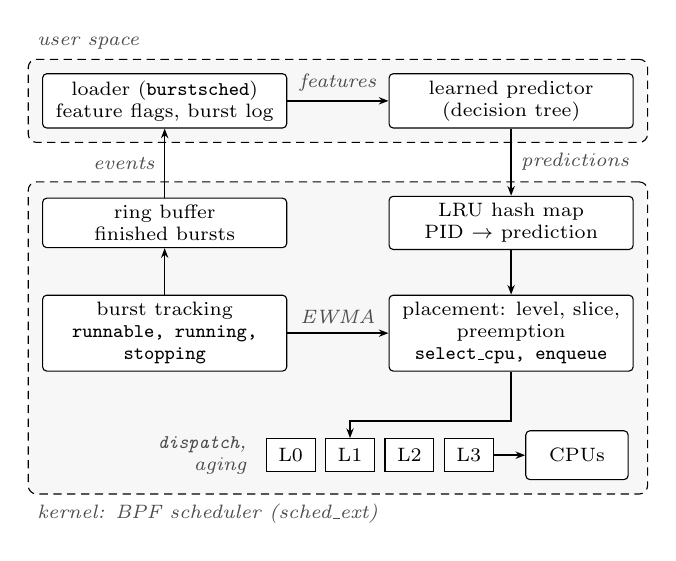
\begin{tikzpicture}[
  font=\scriptsize,
  box/.style={draw, rounded corners=1.5pt, align=center, inner sep=2.5pt,
              minimum height=0.62cm, fill=white},
  q/.style={draw, minimum width=0.62cm, minimum height=0.42cm, inner sep=1pt, fill=white},
  arr/.style={-{Stealth[length=3.5pt]}, semithick},
  lab/.style={font=\scriptsize\itshape, text=black!70}]
  % user space
  \node[box, minimum width=3.1cm] (loader) at (1.75,4.15)
       {loader (\tc{burstsched})\\feature flags, burst log};
  \node[box, minimum width=3.1cm] (tree) at (6.15,4.15)
       {learned predictor\\(decision tree)};
  % kernel objects
  \node[box, minimum width=3.1cm] (rb) at (1.75,2.6) {ring buffer\\finished bursts};
  \node[box, minimum width=3.1cm] (map) at (6.15,2.6) {LRU hash map\\PID $\rightarrow$ prediction};
  \node[box, minimum width=3.1cm] (track) at (1.75,1.2)
       {burst tracking\\\tc{runnable, running,}\\\tc{stopping}};
  \node[box, minimum width=3.1cm] (place) at (6.15,1.2)
       {placement: level, slice,\\preemption\\\tc{select\_cpu, enqueue}};
  % queues
  \node[q] (l0) at (3.35,-0.35) {L0};
  \node[q, right=0.12cm of l0] (l1) {L1};
  \node[q, right=0.12cm of l1] (l2) {L2};
  \node[q, right=0.12cm of l2] (l3) {L3};
  \node[box, minimum width=1.3cm, right=0.4cm of l3] (cpu) {CPUs};
  \node[lab, left=0.12cm of l0, align=right] {\tc{dispatch},\\aging};
  % arrows
  \draw[arr] (track) -- (rb);
  \draw[arr] (rb) -- node[left, lab] {events} (loader);
  \draw[arr] (loader) -- node[above, lab] {features} (tree);
  \draw[arr] (tree) -- node[right, lab] {predictions} (map);
  \draw[arr] (map) -- (place);
  \draw[arr] (track) -- node[above, lab] {EWMA} (place);
  \draw[arr] (place.south) |- ($(l3.north)+(0,0.22)$) -| (l1.north);
  \draw[arr] (l3) -- (cpu);
  % regions
  \begin{scope}[on background layer]
    \node[draw, densely dashed, rounded corners=3pt, fit=(loader)(tree), inner sep=5pt,
          fill=black!3] (user) {};
    \node[draw, densely dashed, rounded corners=3pt, fit=(rb)(map)(track)(place)(l0)(cpu),
          inner sep=5pt, fill=black!3] (kern) {};
  \end{scope}
  \node[lab, anchor=south west] at (user.north west) {user space};
  \node[lab, anchor=north west] at (kern.south west) {kernel: BPF scheduler (sched\_ext)};
\end{tikzpicture}
\caption{Structure of BurstSched. The BPF scheduler measures bursts and places waking tasks in
one of four levels. The loader receives finished bursts through a ring buffer and, with the
learned predictor enabled, returns per-task predictions through a BPF map.}
\label{fig:arch}
\end{figure}

\begin{table}[t]
\caption{Scheduler parameters}
\label{tab:params}
\centering
\footnotesize
\begin{tabular}{@{}lp{4.55cm}@{}}
\toprule
Parameter & Value \\
\midrule
Levels (DSQs) & L0--L3; time slices 2, 4, 8, 16\ms \\
Level of a burst $b$ & L0 if $b<1$\ms, L1 if $b<4$\ms, L2 if $b<12$\ms, else L3 \\
EWMA & $\alpha = 1/8$ (shifts); deviation averaged the same way \\
History before predicting & 3 bursts \\
Confidence test & deviation $<$ 50\% of prediction \\
Predicted slice & $1.25\times$ prediction, clamped to 1--40\ms \\
Ongoing-burst evidence & running $\ge 4$\ms{} without blocking \\
Aging & 100\ms{} without service \\
Preemption & waker at L0 by prediction, target CPU at L2/L3 \\
\bottomrule
\end{tabular}
\end{table}

\subsection{Observing bursts}

When a task starts running, \code{running} records a timestamp; \code{stopping} adds the
elapsed time to the current burst. The callback's \code{runnable} argument tells whether the task
is still runnable (it was preempted or its slice expired) or is blocking. Only in the second
case does the burst end. The task's prediction is then updated and a record is written to a BPF
ring buffer: PID, burst length, the sleep that preceded the burst, the prediction made before
it, the queue wait and the level it was placed at. The \code{runnable} callback measures how long
the task slept. All per-task state lives in BPF task-local storage.

\subsection{Queues and reactive placement}

Each level is a DSQ created by the scheduler, served strictly in priority order. Without
prediction BurstSched is a plain MLFQ: a task that uses its whole slice moves down one level,
and a task that blocks before using half of its slice moves up one level. This configuration
is the reactive baseline in our evaluation.

Starvation is prevented in two ways. \code{dispatch} serves a lower level first if that level
has had work queued but has not been served for 100\ms, and a task that waited longer than
100\ms{} before running is promoted one level.

\subsection{EWMA prediction}

The EWMA predictor implements~(\ref{eq:ewma}) with $\alpha = 1/8$ in integer arithmetic,
$\tau \leftarrow \tau \pm (|t - \tau| \gg 3)$, because BPF has no floating point. It keeps the mean
absolute deviation $\delta$ in the same way. After three bursts, a waking task is placed at the
level that contains its prediction instead of its reactive level.

CPU-bound tasks that never block never finish a burst and would never get a prediction. A
burst still in progress is therefore used as evidence: once a task has run 4\ms{} without
blocking, the scheduler treats it as at least that long.

\subsection{Confidence gating, predicted slices and preemption}

\emph{Confidence gating} acts on a prediction only if $\delta < 0.5\,\tau$; otherwise the task
gets its reactive level. \emph{Predicted slices} replace the fixed slice of each level with
$1.25\,\tau$, clamped to 1--40\ms, so that a CPU-bound task receives a long slice and a short task
a slice just above its burst. \emph{Wakeup preemption} lets a waking task that a prediction
placed at L0 interrupt its target CPU when that CPU is running a task at L2 or L3: the scheduler
calls \code{scx\_bpf\_kick\_cpu} with \code{SCX\_KICK\_PREEMPT}. A task placed by the reactive
rule never preempts, so a wrong guess about an unpredictable task cannot interrupt others.

\subsection{Learned predictor}\label{sec:learned}

The learned predictor runs in the loader. After each finished burst of a task it computes five
features from the task's last two bursts $b_1, b_2$, the sleeps $s_1, s_2$ before them and the
EWMA $e$. With $L(x) \approx \log_2(x+1)$, the features are
\begin{equation}
\begin{aligned}
&L(b_1)-L(e),\quad L(b_1)-L(b_2),\quad L(s_1)-L(b_1),\\
&L(s_2)-L(b_2),\quad L(s_1)-L(s_2).
\end{aligned}
\end{equation}
A decision tree~\cite{cart} trained with scikit-learn~\cite{sklearn} maps these features to one of
three candidates for the next burst: $b_1$, $e$ or $b_2$. The training label is whichever
candidate turned out closest to the real next burst. The predicted burst is the chosen
candidate's value, and the median relative error of the training samples in the chosen leaf
serves as $\delta/\tau$ for the confidence test. The loader writes the prediction and its expected
error into an LRU hash map keyed by PID, and the scheduler uses it in place of the EWMA when an
entry exists.

All features are ratios, so the tree never sees an absolute burst length. We arrived at this
after a failure. Our first version was a regression tree on absolute lengths, and on held-out data it
placed only 32.8\% of the bursts of an unseen periodic task in the right level, against 95.2\%
for the EWMA, because the task's 206\us{} bursts were not among the lengths in the training set
and a regression tree can only output values close to those it was trained on. The candidate
selector has no such limit, since its output is always one of the task's own measurements. The
case it is built for is a phase change: after a 1\,s CPU-bound burst preceded by regular
10\ms{} sleeps, the right answer is the 200\us{} burst before it, $b_2$, which no average over
recent bursts would return.

$L(x)$ is computed as $n + (v - 2^n)/2^n$ with $v = x+1$ and $n = \lfloor\log_2 v\rfloor$, using
the same integer operations in the C loader and in the Python training code, so that both see
identical feature values.

\subsection{Per-CPU queues}

In the per-CPU variant every CPU owns four DSQs, one per level (144 on our machine). A waking task
goes to an idle CPU if \code{scx\_bpf\_select\_cpu\_dfl} finds one. Otherwise a short task (L0
or L1) stays on its previous CPU, where its cache is warm, and a long task is placed by the
power of two choices~\cite{twochoices}: it moves to a random allowed CPU if that CPU has fewer
queued tasks. The same test is applied when a long task's slice expires, because CPU-bound tasks
never wake up and would otherwise never be rebalanced. When a CPU looks for work it goes through
the levels in priority order and, at each level, takes from its own queue before stealing from
the nearest CPU that has a task at that level. Priority is therefore global and locality applies
only within a level.

% ---------------------------------------------------------------------------
\section{Implementation}\label{sec:impl}

The scheduler is about 550 lines of BPF C and the loader about 360 lines of C; the training
script is 180 lines of Python. The build reuses the kernel's own \code{tools/sched\_ext}
Makefile, so libbpf, bpftool and the generated \code{vmlinux.h} always match the running
kernel. Each feature is a read-only BPF variable that the loader sets before loading, so a single
binary covers every configuration. Table~\ref{tab:callbacks} lists the callbacks.

\begin{table}[t]
\caption{sched\_ext callbacks used by BurstSched}
\label{tab:callbacks}
\centering
\footnotesize
\begin{tabular}{@{}lp{5.3cm}@{}}
\toprule
Callback & What BurstSched does \\
\midrule
\code{init} & create the level DSQs (and per-CPU DSQs) \\
\code{init\_task} & allocate task-local storage \\
\code{select\_cpu} & idle CPU: dispatch directly; per-CPU mode: affinity or two choices \\
\code{enqueue} & choose level and slice, insert, maybe kick a CPU to preempt \\
\code{dispatch} & aging, then highest non-empty level; per-CPU: own queue, then steal \\
\code{runnable} & end of sleep: record sleep length \\
\code{running} & start of a run: timestamp, queue wait, aging promotion \\
\code{stopping} & accumulate burst; if blocking, update prediction and log the burst \\
\bottomrule
\end{tabular}
\end{table}

A small tool, \code{setext}, runs a command under the \code{SCHED\_EXT} policy so that we could
develop in partial mode without disturbing other users of the shared lab machine. A second BPF
program, \code{waitmon}, attaches to the \code{sched\_wakeup}, \code{sched\_wakeup\_new} and
\code{sched\_switch} tracepoints and records how long each task stays runnable without running.
Because it observes the core scheduler rather than our callbacks, it measures EEVDF,
\code{scx\_simple} and BurstSched in the same way.

Three problems during development changed the design. First, in full mode the loader is itself
scheduled by BurstSched, so every time it blocked it produced a burst record, which woke it up
again. One run of the steady workload, about 35\,s long, produced 12.3 million context switches. Filtering out the loader's own
process and having the loader drain the ring buffer every 2\ms{} instead of being woken for
each record brought this down to 53 thousand. Second, the first per-CPU version balanced load
only when a task woke up. CPU hogs never wake up, so the imbalance it started with persisted:
Jain's fairness index over the hogs' CPU time~\cite{jain} was 0.967, and one task waited
164\ms.
Rebalancing long tasks when their slice expires and stealing by priority level raised the index
to 0.9994 and lowered that wait to 82\ms. Third, the regression-tree predictor described in
Section~\ref{sec:learned} had to be replaced.

% ---------------------------------------------------------------------------
\section{Experimental setup}\label{sec:method}

All results come from one 36-CPU x86-64 workstation running Ubuntu 24.04 with kernel
6.17.0. Development used a second workstation of the same size with kernel 7.0. During every
measurement, 72 \code{stress-ng}~\cite{stressng} CPU workers (two per CPU) provide background
load, and all tasks on the machine, including system threads, are scheduled by the scheduler
under test (full mode). Each configuration was run three times; we report the median of the three
runs.

\textbf{Workloads.} \emph{Steady:} \code{wakeup\_lat} sleeps until an absolute deadline every
10\ms, measures how late it starts running, and then computes for 200\us; 3000 iterations. Timer
slack is set to 1\,ns so that the measurement contains scheduling delay only.
\emph{Phase change:} \code{phase\_change} alternates 10 times between 2\,s of computation and
2\,s of the steady pattern. We report latency over all wakeups, \emph{recovery} latency over the
first 10 wakeups after each CPU phase (cycles 2--10), and the very first wakeup of the run
(\emph{cold start}). \emph{Request/response:} \code{rr\_bench} runs a server process that answers
64-byte requests over loopback TCP after 100\us{} of computation; four client threads each send
200 requests per second on a fixed schedule, and latency is measured from the scheduled send time
to the reply.

\textbf{Configurations.} Table~\ref{tab:configs} lists them. The BurstSched configurations add
one feature at a time; \emph{learned} replaces the EWMA of \emph{full} with the learned
predictor.

\begin{table}[t]
\caption{Configurations}
\label{tab:configs}
\centering
\footnotesize
\begin{tabular}{@{}lp{5.05cm}@{}}
\toprule
Name & Scheduler and features \\
\midrule
EEVDF & default Linux scheduler, no BPF scheduler loaded \\
scx\_simple & example sched\_ext scheduler, one global vtime queue \\
MLFQ & BurstSched, reactive placement and aging only \\
+ EWMA & placement by EWMA prediction \\
+ confidence & EWMA with confidence gating \\
+ pred.\ slices & time slice scaled to the prediction \\
+ preemption & wakeup preemption (``full'' EWMA design) \\
+ learned & learned predictor instead of EWMA \\
+ per-CPU & per-CPU queues, two choices, work stealing \\
\bottomrule
\end{tabular}
\end{table}

\textbf{Metrics.} Wakeup and request latency (p50, p99, maximum); CPU-hog throughput in
\code{stress-ng} bogo operations per second; system-wide context switches from
\code{/proc/stat}; Jain's index~\cite{jain} over the CPU time of the 72 hogs; and worst-case
wait from \code{waitmon}, both for the hogs and for the measured task.

The learned predictor was trained once, on burst logs from workloads with different parameters
than the test workloads (other sleep intervals, burst lengths and phase lengths, a pipe stressor
and partially loaded CPU workers). After limiting each task to 3000 samples, the training set had
44{,}788 samples. The resulting tree has depth~5 and 39 nodes, and it was not retrained for any
experiment.

% ---------------------------------------------------------------------------
\section{Results}\label{sec:results}

\begin{figure*}[t]
\centering
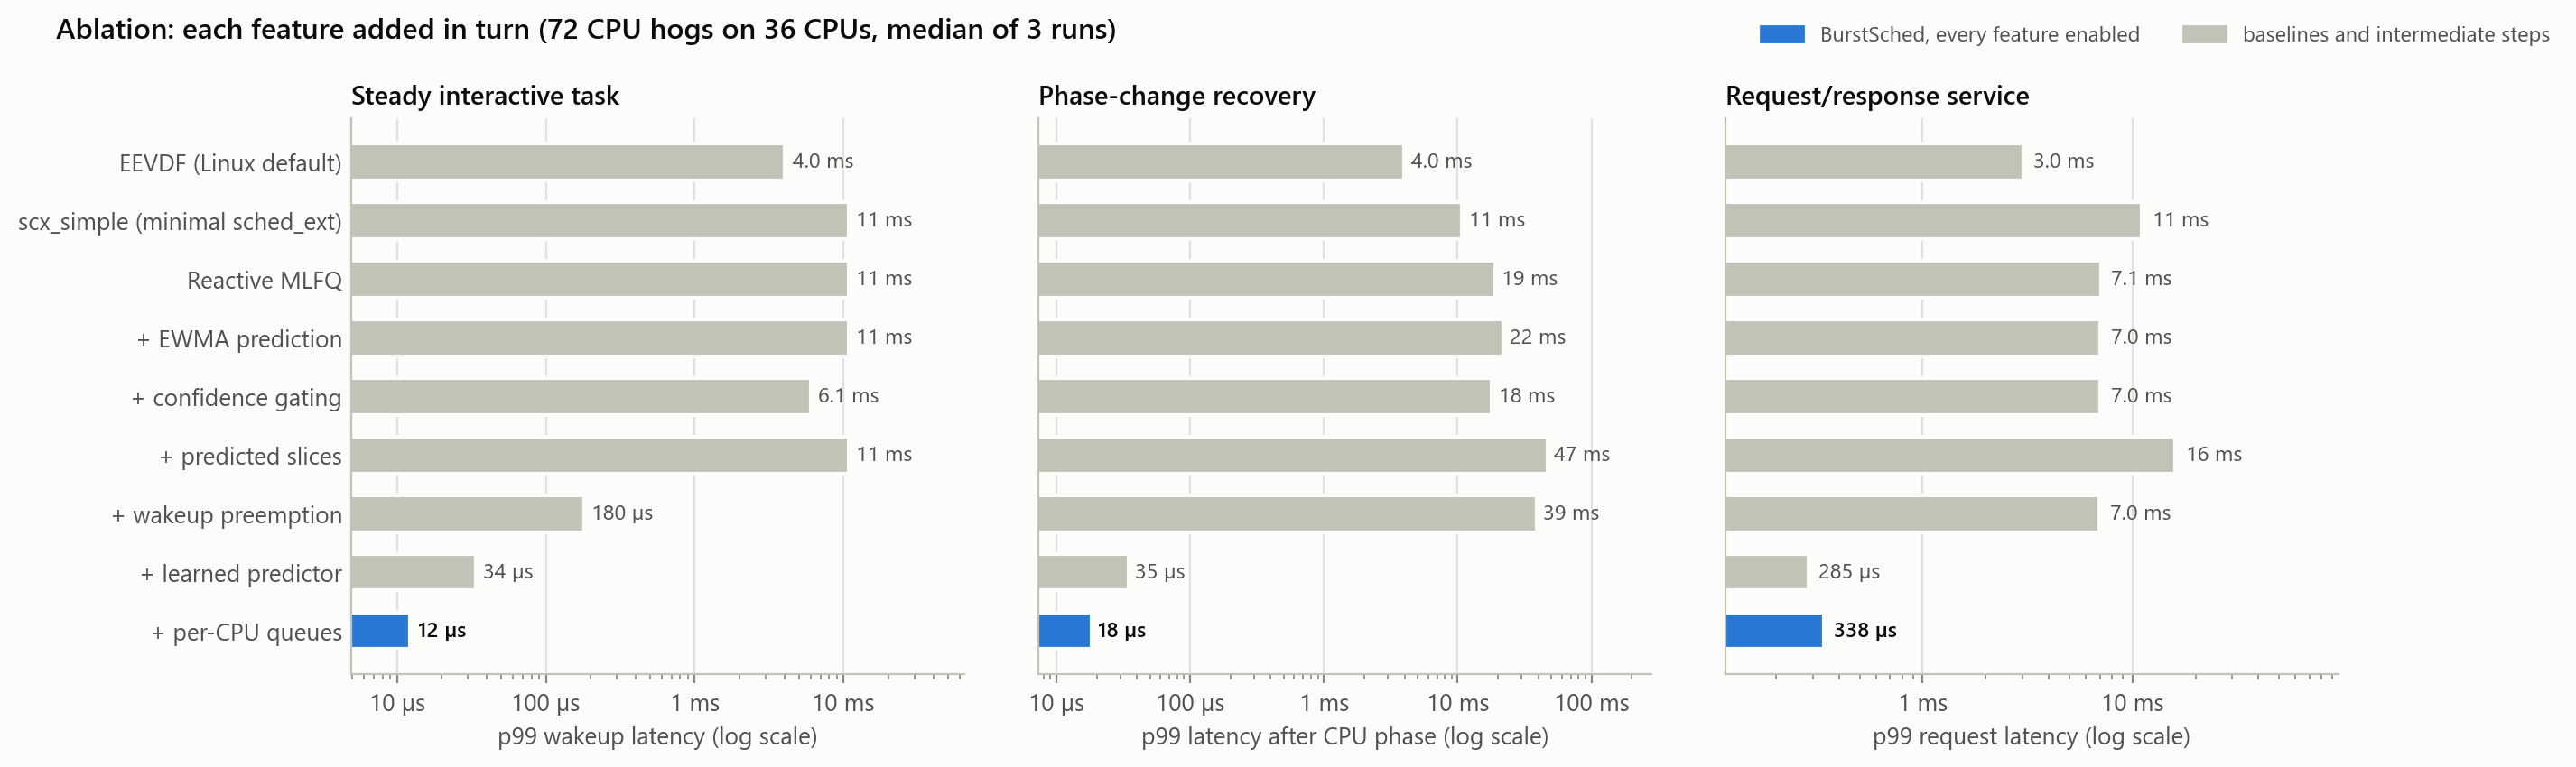
\includegraphics[width=\textwidth]{fig1_ablation}
\caption{Ablation over the nine configurations (median of three runs, log scale). (a) p99 wakeup
latency of the steady task. (b) p99 latency of the first ten wakeups after each CPU-bound phase.
(c) p99 latency of the request/response service.}
\label{fig:ablation}
\end{figure*}

Fig.~\ref{fig:ablation} summarizes the ablation and Table~\ref{tab:summary} compares the two
baselines, the reactive MLFQ and BurstSched with every feature enabled.

\begin{table}[t]
\caption{Baselines and full BurstSched (median of three runs)}
\label{tab:summary}
\centering
\footnotesize
\setlength{\tabcolsep}{3.2pt}
\begin{tabular}{@{}lrrrr@{}}
\toprule
 & EEVDF & scx\_simple & MLFQ & BurstSched \\
\midrule
Steady task, p99 & 4.0\ms & 10.8\ms & 10.8\ms & 12\us \\
Phase recovery, p99 & 4.0\ms & 10.8\ms & 19.0\ms & 18\us \\
Request/response, p99 & 3.0\ms & 11.1\ms & 7.1\ms & 338\us \\
Requests completed & 99.9\% & 51.8\% & 59.9\% & 100\% \\
Context switches (steady) & 339k & 73k & 87k & 56k \\
Hog throughput (ops/s) & 63.5k & 63.5k & 63.5k & 63.6k \\
Jain index (steady) & 0.9935 & 1.0000 & 1.0000 & 0.9999 \\
Worst hog wait (steady) & 20\ms & 62\ms & 23\ms & 82\ms \\
\bottomrule
\end{tabular}
\end{table}

\subsection{Steady interactive task}

EEVDF has the lowest median wakeup latency of all configurations, 6.8\us, but its distribution
has two modes (Fig.~\ref{fig:tail}): 17.7\% of wakeups wait more than 1\ms, and the p99 is
4.0\ms. Reactive MLFQ places the task in L0 every time, yet its median is 805\us{} and its p99
10.8\ms, because a task at L0 still has to wait until some CPU finishes the time slice of a hog.
Adding the EWMA does not change this, and confidence gating helps only a little (p99 6.1\ms).
Predicted slices make it worse again, since hog slices grow to 40\ms.

\begin{figure}[t]
\centering
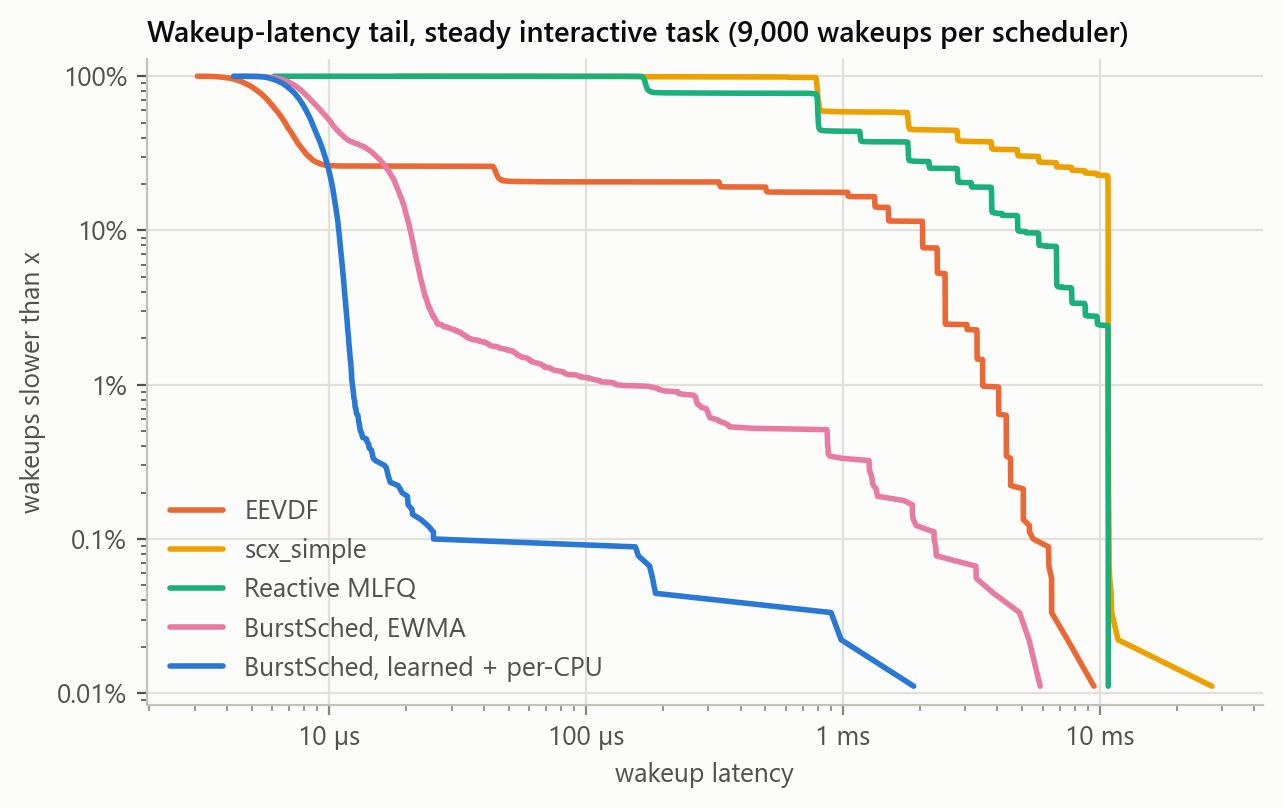
\includegraphics[width=\columnwidth]{fig2_wakeup_tail}
\caption{Share of the 9000 wakeups of the steady task (three runs) that took longer than a given
latency.}
\label{fig:tail}
\end{figure}

Wakeup preemption is what changes the picture: p99 falls from 10.8\ms{} to 180\us{} and only
0.32\% of wakeups wait more than 1\ms. The learned predictor lowers p99 further to 34\us, and
per-CPU queues to 12\us, with a single wakeup out of 9000 above 1\ms.

\subsection{Phase changes}

After each 2\,s CPU-bound phase, the reactive MLFQ finds the task at L3. The median latency of
the first wakeup after a phase is 17.8\ms; from the second wakeup on it is back to the same
800\us{} as in the steady case (Fig.~\ref{fig:recovery}). The EWMA does not help here: after a
1\,s burst the average is near 125\ms{} and the deviation is as large, so confidence gating
rejects it and the task falls back to its reactive level. With predicted slices and preemption the
first wakeup costs even more, 34.6\ms{} at the median, because the task now waits behind hogs
whose slices have grown to 40\ms. EEVDF handles this case well; its recovery latency is the same
as in the steady state.

\begin{figure}[t]
\centering
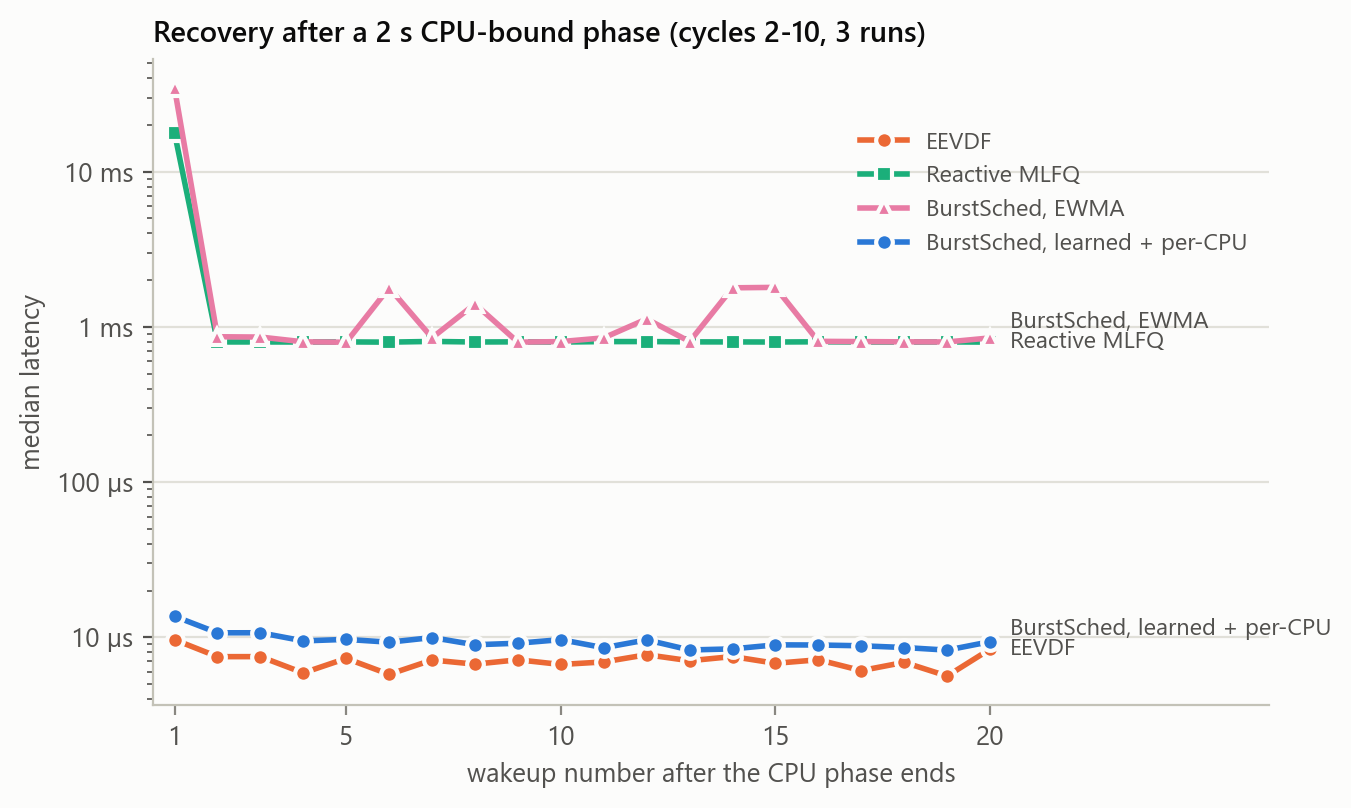
\includegraphics[width=\columnwidth]{fig3_phase_recovery}
\caption{Median latency of the $n$-th wakeup after a 2\,s CPU-bound phase (cycles 2--10, three
runs).}
\label{fig:recovery}
\end{figure}

The learned predictor picks the burst before the long one and places the task at L0 on its first
wakeup, where it is allowed to preempt. The first wakeup takes 13\us{} at the median, and recovery
p99 falls from 39.0\ms{} to 35\us{} (18\us{} with per-CPU queues). Table~\ref{tab:misplace}
counts the placements directly from the burst logs. With the EWMA or reactive placement, 1.5\%
of the phase task's bursts were queued below their level, about three after every CPU phase,
each waiting 22--48\ms{} at p99. With the learned predictor there were none, and with per-CPU
queues two in total over the three runs.

\begin{table}[t]
\caption{Phase task: bursts queued below their level}
\label{tab:misplace}
\centering
\footnotesize
\begin{tabular}{@{}lrr@{}}
\toprule
Configuration & Queued too low & p99 wait of those \\
\midrule
MLFQ & 1.5\% & 22\ms \\
+ EWMA & 1.5\% & 23\ms \\
+ confidence & 1.5\% & 22\ms \\
+ pred.\ slices & 1.6\% & 48\ms \\
+ preemption & 1.5\% & 39\ms \\
+ learned & 0.0\% & none \\
+ per-CPU & 0.03\% & 5\ms \\
\bottomrule
\end{tabular}
\end{table}

\emph{Cold start.} The very first CPU-to-interactive switch of a process can only be predicted
from whatever the process did before. In full mode the bursts of process start-up provide enough
history, and the first wakeup took 25\us{} with the learned predictor (median of three runs).
With per-CPU queues the three runs gave 11\us, 2.0\ms{} and 5.0\ms. In an earlier experiment in
partial mode, where the task joined the scheduler immediately before its first CPU phase, the
same wakeup took 42\ms{} because there was no history at all.

\subsection{Request/response service}

This workload separates the two predictors more clearly than the others
(Fig.~\ref{fig:ablation}c). With the EWMA, p99 stays at 7.0\ms{} even with preemption enabled;
with the learned predictor it is 285\us, and 338\us{} with per-CPU queues. EEVDF reaches
3.0\ms. Several configurations could not keep up with the offered 800 requests per second: the
clients skip requests when they fall behind schedule, and reactive MLFQ completed only 59.9\% of
them, \code{scx\_simple} 51.8\% and the full EWMA design 94.4\%, against 100\% for the learned
predictor. The latency percentiles of those configurations cover only the requests that were
sent, so they understate the difference.

\begin{table}[t]
\caption{Why the EWMA does not trigger preemption for the request/response clients
(full EWMA design, one run)}
\label{tab:rr}
\centering
\footnotesize
\setlength{\tabcolsep}{3pt}
\begin{tabular}{@{}lccc@{}}
\toprule
Thread & Burst p10/p50/p90 & $\delta/\tau$ & Passes confidence test \\
\midrule
server & 112/116/121\us & 0.03 & 100\% \\
clients & 4/8/30\us & 0.66 & 1\% \\
\bottomrule
\end{tabular}
\end{table}

Table~\ref{tab:rr} shows the cause. The server's bursts are regular and its EWMA passes the
confidence test. The client threads' bursts are tiny but vary by a factor of seven, so their
deviation is large \emph{relative to the prediction} and the test rejects it. The clients are
still queued at L0, the correct level, but because the reactive rule placed them they may not
preempt, and each of their wakeups waits for a hog's slice to end. The learned predictor's leaf
error for this pattern is small, so 99.9\% of client bursts were placed by prediction and could
preempt. The confidence test is measuring the wrong thing: a burst between 4 and 30\us{} is
certainly below the 1\ms{} boundary of L0, and that is all the placement needs to know.

\subsection{Costs}

\begin{figure*}[t]
\centering
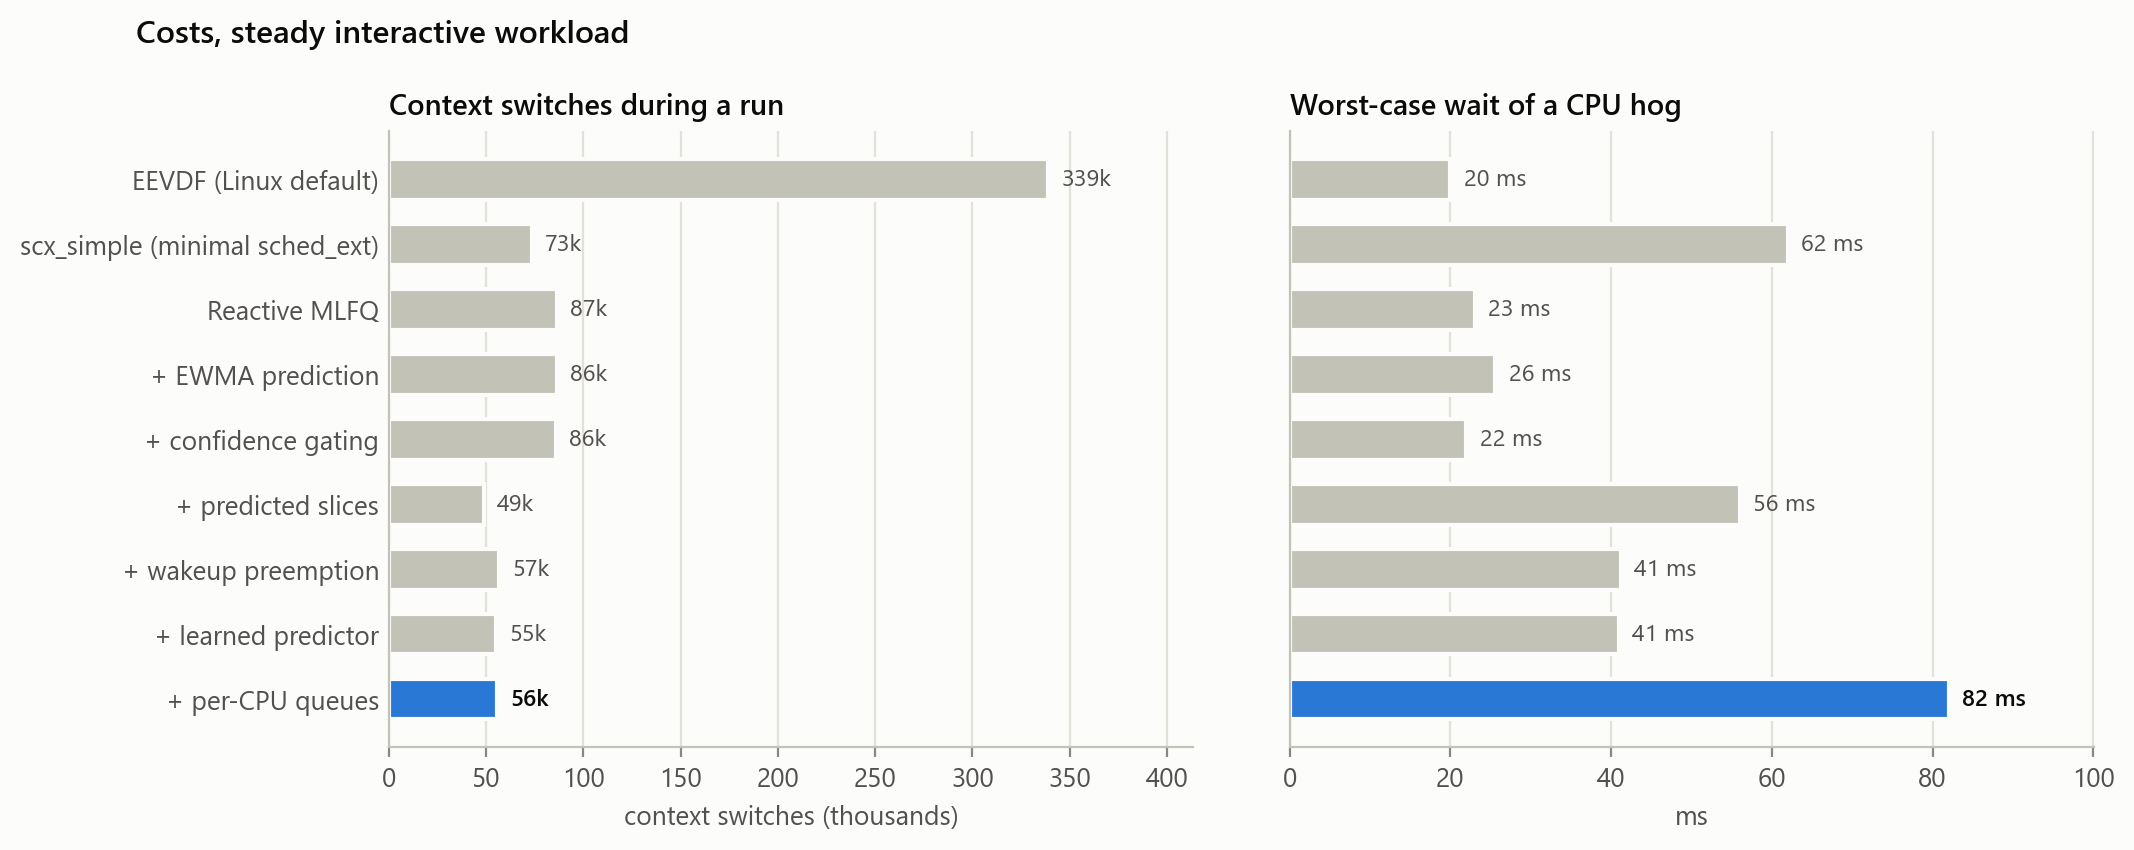
\includegraphics[width=\textwidth]{fig4_costs}
\caption{Costs in the steady workload. (a) System-wide context switches during a run. (b) Longest
time any CPU hog was runnable without running, measured by \code{waitmon}.}
\label{fig:costs}
\end{figure*}

Fig.~\ref{fig:costs} shows what the latency gains cost. BurstSched with every feature enabled
caused 56 thousand context switches in a run of the steady workload, against 339 thousand under
EEVDF; for the phase and request/response workloads the ratios are 6.4 and 2.9. Most of the
difference comes from the 16--40\ms{} slices given to CPU-bound tasks: reactive MLFQ with fixed
16\ms{} slices already needs only 87 thousand, and adding predicted slices halves the count again
(86 to 49 thousand). Each run caused about 10 thousand preemptions in the
steady workload and 30 thousand in the request/response workload. Hog throughput was within
0.5\% across all configurations of a workload, so neither the preemptions nor the BPF scheduler
itself had a measurable effect on batch work.

The hogs' share of CPU time stayed even: Jain's index was at least 0.9997 for every BurstSched
configuration, compared with 0.990--0.994 for EEVDF. The longest single wait of a hog is a
different matter. It was 20\ms{} under EEVDF and 23\ms{} under reactive MLFQ, 56\ms{} once
predicted slices were added, 41\ms{} with preemption on top, and 82\ms{} with per-CPU queues. Long slices and interactive
tasks jumping the queue both delay the next hog in line, and with per-CPU queues a hog can wait
behind the slices of the other hogs on its own CPU before any other CPU steals it.

\subsection{Predictor accuracy}

\begin{figure*}[t]
\centering
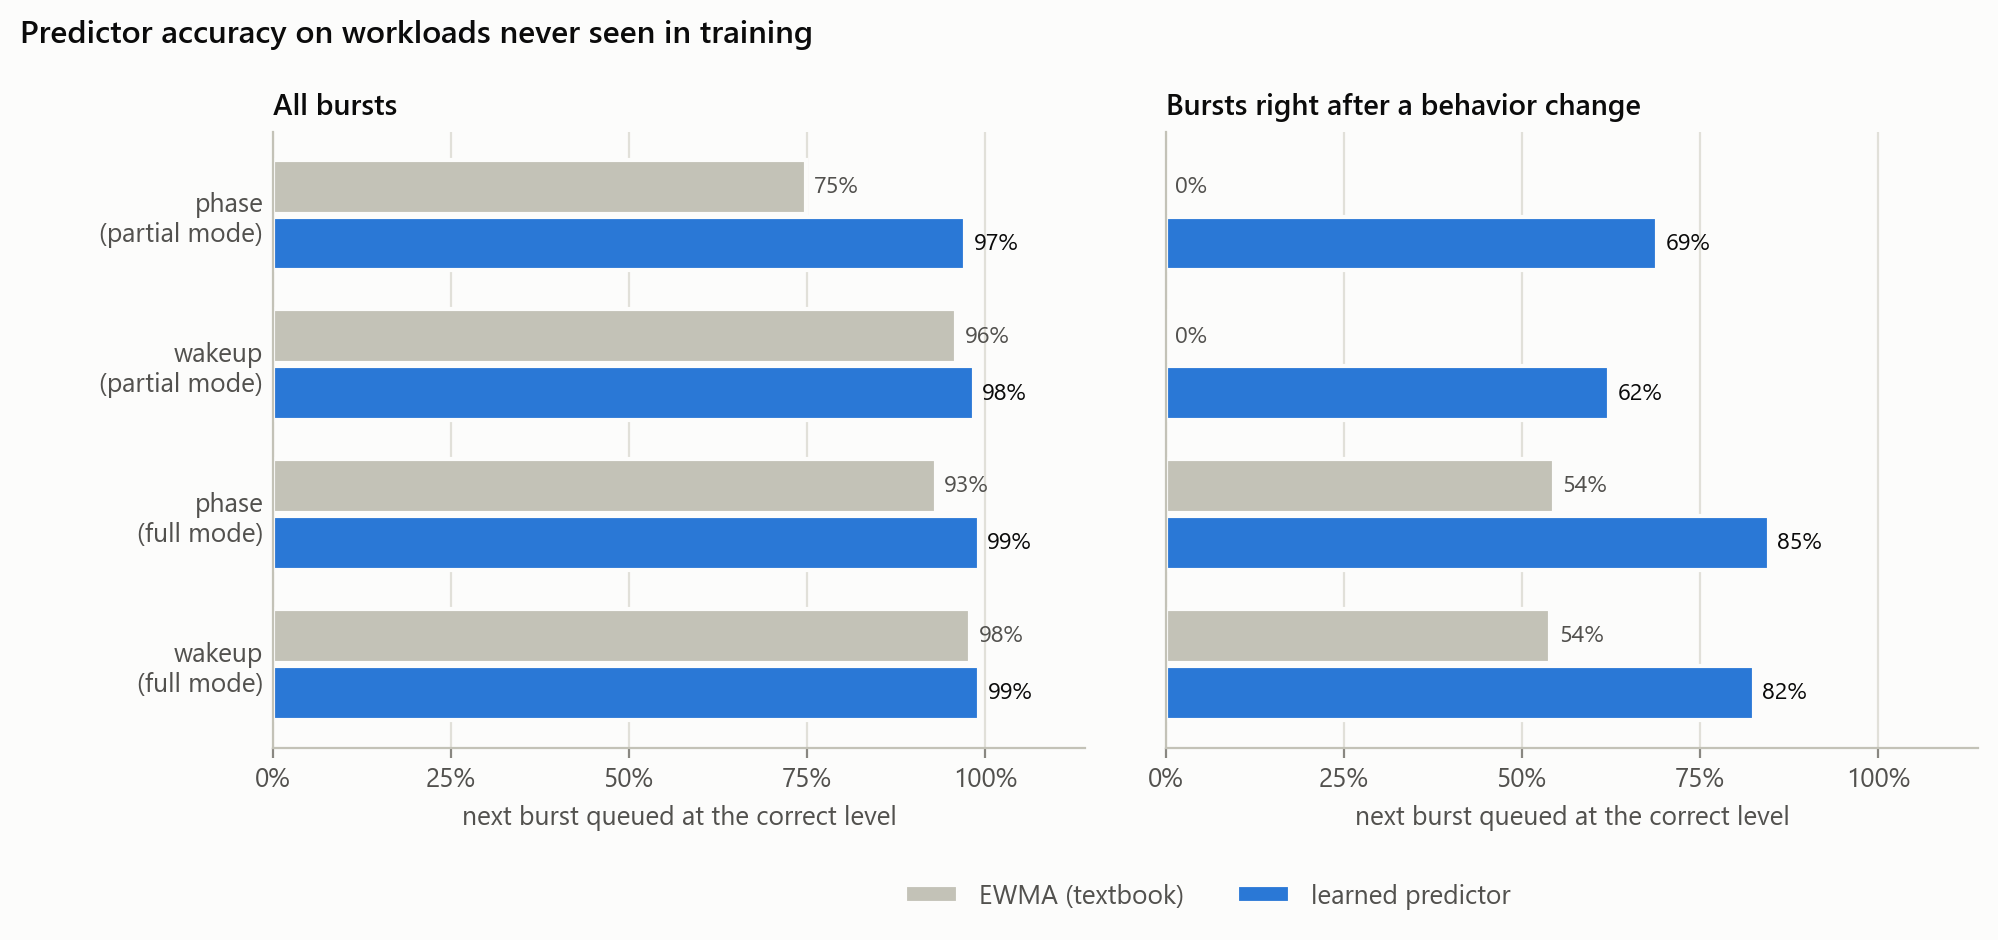
\includegraphics[width=\textwidth]{fig5_predictor}
\caption{Share of next bursts placed in the correct level, on burst logs not used for training.
(a) All bursts. (b) Bursts whose predecessor differed by a factor of 8 or more from the burst
before it.}
\label{fig:predictor}
\end{figure*}

Fig.~\ref{fig:predictor} evaluates both predictors offline on four burst logs that were not used
in training: the phase and steady workloads from an early partial-mode run, which contain only
the measured task and the hogs, and from a full-mode run, which contain every task on the
machine. Over all
bursts the learned predictor chose the correct level for 97--99\% of bursts, against 75--98\%
for the EWMA. The difference is concentrated where behavior changes. On bursts that follow a
change of a factor of 8 or more, the EWMA was right 0\% of the time for the measured tasks and
54\% for all tasks; the learned predictor was right 62--69\% and 82--85\% of the time. The most
important features were the ratio of the last burst to the EWMA (importance 0.38) and of the last
burst to the one before (0.32).

\subsection{Which features mattered}

Reading Fig.~\ref{fig:ablation} from top to bottom: the EWMA alone changed nothing measurable;
confidence gating helped the steady task; predicted slices halved context switches but hurt
latency until preemption was added; preemption produced the largest single improvement for the
steady task but none for phase changes or the request/response clients; the learned predictor
fixed both of those; per-CPU queues improved the steady and phase workloads further, made the
request/response service slightly slower (285\us{} to 338\us{} at p99, in all three runs) and
doubled the worst hog wait.

% ---------------------------------------------------------------------------
\section{Discussion and limitations}\label{sec:discussion}

\textbf{Placement versus preemption.} Every configuration put the steady task and the
request/response threads in the correct level for 100\% of their bursts, and yet their p99
latency ranged from 12\us{} to 11\ms. Under load, a correctly placed task still waits for a CPU,
and the queue it sits in only decides how long. In our results prediction pays off through the
decisions that depend on it, mainly which waking tasks may preempt, more than through placement
itself.

\textbf{The confidence test.} Measuring confidence relative to the prediction is wrong for very
short bursts. A test that asks whether $\tau + 2\delta$ stays below the boundary of the predicted
level would have accepted the request/response clients. We did not have time to evaluate it.

\textbf{Worst-case wait.} BurstSched trades the longest wait of CPU-bound tasks for interactive
latency. For batch jobs on a server that trade is usually acceptable; for a CPU-bound task that
must meet a deadline, 82\ms{} may not be.

\textbf{Scope of the evaluation.} We used three synthetic workloads, one machine and three runs
per configuration, with CPU-bound background load. We did not measure a desktop session, a
compile job, a multi-socket machine or memory-bound background load, and we did not measure the
CPU cost of the BPF callbacks separately; the unchanged hog throughput only bounds it. The
learned predictor was trained once, offline. The phase-change workload resembles part of its
training data in structure, though with different durations, burst lengths and sleep intervals;
the request/response workload does not.

% ---------------------------------------------------------------------------
\section{Related work}\label{sec:related}

The MLFQ goes back to CTSS~\cite{corbato} and is the basis of the schedulers of several Unix
systems; ULE~\cite{ule} computes an interactivity score from recent sleep and run time, which is
an implicit burst estimate. Linux replaced CFS with EEVDF~\cite{eevdf,eevdfdoc}, which provides
proportional sharing with latency control through per-task slices rather than through task
classification.

Work on microsecond-scale tail latency for datacenter services, such as Shinjuku~\cite{shinjuku}
and Shenango~\cite{shenango}, also relies on fast preemption and fine-grained core reallocation,
but in dedicated systems rather than in the general-purpose kernel scheduler. ghOSt~\cite{ghost}
delegates scheduling decisions to user-space agents; sched\_ext~\cite{schedext} instead runs the
policy itself in BPF inside the kernel, and its repository contains schedulers that also try to
recognize latency-critical tasks, for example from how often they wake up and
block~\cite{scx}. Learned scheduling has been applied mostly to cluster schedulers, as in
Decima~\cite{decima}. BurstSched keeps the learned component small and interpretable and lets the
kernel consume only its output.

% ---------------------------------------------------------------------------
\section{Conclusion}\label{sec:conclusion}

BurstSched shows that burst prediction can be added to a multilevel feedback queue on an
unmodified Linux kernel and that it can lower interactive tail latency by two orders of
magnitude under heavy CPU load without losing batch throughput. The textbook EWMA, however,
contributed little on its own. The gains came from what the prediction was used for, chiefly
deciding which waking tasks may preempt, and from a learned predictor that recognizes a change of
behavior from the task's own recent history. The main open problems are a confidence test that
reasons about queue levels instead of relative error, and the longer worst-case wait of
CPU-bound tasks.

\section*{Code and data}

Source code, the trained model, the measurement data and the scripts that produce every figure
and table are available at \url{https://github.com/lakshya-74/BurstSched}.

% ---------------------------------------------------------------------------
% balance the two columns of the last page
\IEEEtriggeratref{11}
\begin{thebibliography}{99}

\bibitem{silberschatz}
A.~Silberschatz, P.~B. Galvin, and G.~Gagne, \emph{Operating System Concepts}, 10th~ed.
Hoboken, NJ, USA: Wiley, 2018.

\bibitem{corbato}
F.~J. Corbat\'{o}, M.~Merwin-Daggett, and R.~C. Daley, ``An experimental time-sharing system,''
in \emph{Proc. AFIPS Spring Joint Comput. Conf.}, 1962, pp.~335--344.

\bibitem{ostep}
R.~H. Arpaci-Dusseau and A.~C. Arpaci-Dusseau, \emph{Operating Systems: Three Easy Pieces}.
Arpaci-Dusseau Books, 2018, ch.~8, ``Scheduling: The multi-level feedback queue.''

\bibitem{schedext}
``Extensible scheduler class,'' \emph{The Linux Kernel Documentation}. [Online]. Available:
\url{https://docs.kernel.org/scheduler/sched-ext.html}

\bibitem{eevdf}
I.~Stoica and H.~Abdel-Wahab, ``Earliest eligible virtual deadline first: A flexible and accurate
mechanism for proportional share resource allocation,'' Old Dominion Univ., Norfolk, VA, USA,
Tech. Rep. TR-95-22, 1995.

\bibitem{eevdfdoc}
``EEVDF scheduler,'' \emph{The Linux Kernel Documentation}. [Online]. Available:
\url{https://docs.kernel.org/scheduler/sched-eevdf.html}

\bibitem{bpfdoc}
``BPF documentation,'' \emph{The Linux Kernel Documentation}. [Online]. Available:
\url{https://docs.kernel.org/bpf/}

\bibitem{ule}
J.~Roberson, ``ULE: A modern scheduler for FreeBSD,'' in \emph{Proc. BSDCon}, 2003.

\bibitem{cart}
L.~Breiman, J.~H. Friedman, R.~A. Olshen, and C.~J. Stone, \emph{Classification and Regression
Trees}. Belmont, CA, USA: Wadsworth, 1984.

\bibitem{sklearn}
F.~Pedregosa \emph{et al.}, ``Scikit-learn: Machine learning in Python,'' \emph{J. Mach. Learn.
Res.}, vol.~12, pp.~2825--2830, 2011.

\bibitem{twochoices}
M.~Mitzenmacher, ``The power of two choices in randomized load balancing,'' \emph{IEEE Trans.
Parallel Distrib. Syst.}, vol.~12, no.~10, pp.~1094--1104, Oct. 2001.

\bibitem{jain}
R.~Jain, D.-M. Chiu, and W.~R. Hawe, ``A quantitative measure of fairness and discrimination for
resource allocation in shared computer systems,'' Digital Equipment Corp., Tech. Rep. DEC-TR-301,
1984.

\bibitem{stressng}
C.~I. King, ``stress-ng.'' [Online]. Available: \url{https://github.com/ColinIanKing/stress-ng}

\bibitem{shinjuku}
K.~Kaffes \emph{et al.}, ``Shinjuku: Preemptive scheduling for $\mu$second-scale tail latency,''
in \emph{Proc. 16th USENIX Symp. Networked Syst. Design Implement. (NSDI)}, 2019.

\bibitem{shenango}
A.~Ousterhout, J.~Fried, J.~Behrens, A.~Belay, and H.~Balakrishnan, ``Shenango: Achieving high CPU
efficiency for latency-sensitive datacenter workloads,'' in \emph{Proc. 16th USENIX Symp.
Networked Syst. Design Implement. (NSDI)}, 2019.

\bibitem{ghost}
J.~T. Humphries \emph{et al.}, ``ghOSt: Fast \& flexible user-space delegation of Linux
scheduling,'' in \emph{Proc. 28th ACM Symp. Operating Syst. Principles (SOSP)}, 2021.

\bibitem{scx}
``sched\_ext schedulers and tools.'' [Online]. Available: \url{https://github.com/sched-ext/scx}

\bibitem{decima}
H.~Mao, M.~Schwarzkopf, S.~B. Venkatakrishnan, Z.~Meng, and M.~Alizadeh, ``Learning scheduling
algorithms for data processing clusters,'' in \emph{Proc. ACM SIGCOMM}, 2019.

\end{thebibliography}

\end{document}
